%!TEX TS-program = xelatex

% Шаблон документа LaTeX создан в 2018 году
% Алексеем Подчезерцевым
% В качестве исходных использованы шаблоны
% 	Данилом Фёдоровых (danil@fedorovykh.ru) 
%		https://www.writelatex.com/coursera/latex/5.2.2
%	LaTeX-шаблон для русской кандидатской диссертации и её автореферата.
%		https://github.com/AndreyAkinshin/Russian-Phd-LaTeX-Dissertation-Template

\documentclass[a4paper,14pt]{article}


%%% Работа с русским языком
\usepackage[english,russian]{babel}   %% загружает пакет многоязыковой вёрстки
\usepackage{fontspec}      %% подготавливает загрузку шрифтов Open Type, True Type и др.
\defaultfontfeatures{Ligatures={TeX},Renderer=Basic}  %% свойства шрифтов по умолчанию
\setmainfont[Ligatures={TeX,Historic}]{Times New Roman} %% задаёт основной шрифт документа
\setsansfont{Comic Sans MS}                    %% задаёт шрифт без засечек
\setmonofont{Courier New}
\usepackage{indentfirst}
\frenchspacing

\renewcommand{\epsilon}{\ensuremath{\varepsilon}}
\renewcommand{\phi}{\ensuremath{\varphi}}
\renewcommand{\kappa}{\ensuremath{\varkappa}}
\renewcommand{\le}{\ensuremath{\leqslant}}
\renewcommand{\leq}{\ensuremath{\leqslant}}
\renewcommand{\ge}{\ensuremath{\geqslant}}
\renewcommand{\geq}{\ensuremath{\geqslant}}
\renewcommand{\emptyset}{\varnothing}

%%% Дополнительная работа с математикой
\usepackage{amsmath,amsfonts,amssymb,amsthm,mathtools} % AMS
\usepackage{icomma} % "Умная" запятая: $0,2$ --- число, $0, 2$ --- перечисление

%% Номера формул
%\mathtoolsset{showonlyrefs=true} % Показывать номера только у тех формул, на которые есть \eqref{} в тексте.
%\usepackage{leqno} % Нумерация формул слева	

%% Перенос знаков в формулах (по Львовскому)
\newcommand*{\hm}[1]{#1\nobreak\discretionary{}
	{\hbox{$\mathsurround=0pt #1$}}{}}

%%% Работа с картинками
\usepackage{graphicx}  % Для вставки рисунков
\graphicspath{{images/}}  % папки с картинками
\setlength\fboxsep{3pt} % Отступ рамки \fbox{} от рисунка
\setlength\fboxrule{1pt} % Толщина линий рамки \fbox{}
\usepackage{wrapfig} % Обтекание рисунков текстом

%%% Работа с таблицами
\usepackage{array,tabularx,tabulary,booktabs} % Дополнительная работа с таблицами
\usepackage{longtable}  % Длинные таблицы
\usepackage{multirow} % Слияние строк в таблице
\usepackage{float}% http://ctan.org/pkg/float

%%% Программирование
\usepackage{etoolbox} % логические операторы


%%% Страница
\usepackage{extsizes} % Возможность сделать 14-й шрифт
\usepackage{geometry} % Простой способ задавать поля
\geometry{top=20mm}
\geometry{bottom=20mm}
\geometry{left=20mm}
\geometry{right=10mm}
%
%\usepackage{fancyhdr} % Колонтитулы
% 	\pagestyle{fancy}
%\renewcommand{\headrulewidth}{0pt}  % Толщина линейки, отчеркивающей верхний колонтитул
% 	\lfoot{Нижний левый}
% 	\rfoot{Нижний правый}
% 	\rhead{Верхний правый}
% 	\chead{Верхний в центре}
% 	\lhead{Верхний левый}
%	\cfoot{Нижний в центре} % По умолчанию здесь номер страницы

\usepackage{setspace} % Интерлиньяж
\onehalfspacing % Интерлиньяж 1.5
%\doublespacing % Интерлиньяж 2
%\singlespacing % Интерлиньяж 1

\usepackage{lastpage} % Узнать, сколько всего страниц в документе.

\usepackage{soul} % Модификаторы начертания

\usepackage{hyperref}
\usepackage[usenames,dvipsnames,svgnames,table,rgb]{xcolor}
\hypersetup{				% Гиперссылки
	unicode=true,           % русские буквы в раздела PDF
	pdftitle={Заголовок},   % Заголовок
	pdfauthor={Автор},      % Автор
	pdfsubject={Тема},      % Тема
	pdfcreator={Создатель}, % Создатель
	pdfproducer={Производитель}, % Производитель
	pdfkeywords={keyword1} {key2} {key3}, % Ключевые слова
	colorlinks=true,       	% false: ссылки в рамках; true: цветные ссылки
	linkcolor=black,          % внутренние ссылки
	citecolor=black,        % на библиографию
	filecolor=magenta,      % на файлы
	urlcolor=black           % на URL
}
\makeatletter 
\def\@biblabel#1{#1. } 
\makeatother
\usepackage{cite} % Работа с библиографией
%\usepackage[superscript]{cite} % Ссылки в верхних индексах
%\usepackage[nocompress]{cite} % 
\usepackage{csquotes} % Еще инструменты для ссылок

\usepackage{multicol} % Несколько колонок

\usepackage{tikz} % Работа с графикой
\usepackage{pgfplots}
\usepackage{pgfplotstable}

% ГОСТ заголовки
\usepackage[font=small]{caption}
%\captionsetup[table]{justification=centering, labelsep = newline} % Таблицы по правобу краю
%\captionsetup[figure]{justification=centering} % Картинки по центру


\newcommand{\tablecaption}[1]{\addtocounter{table}{1}\small \begin{flushright}\tablename \ \thetable\end{flushright}%	
\begin{center}#1\end{center}}

\newcommand{\imref}[1]{рис.~\ref{#1}}

\usepackage{multirow}
\usepackage{spreadtab}
\newcolumntype{K}[1]{@{}>{\centering\arraybackslash}p{#1cm}@{}}


\usepackage{xparse}
\ExplSyntaxOn
\DeclareExpandableDocumentCommand{\juliandate}{ m m m }
{
	\juliandate_calc:nnnn { #1 } { #2 } { #3 } { \use:n }
}
\NewDocumentCommand{\storejuliandate}{ s m m m m }
{
	\IfBooleanTF{#1}
	{
		\juliandate_calc:nnnn { #3 } { #4 } { #5 } { \cs_set:Npx #2 }
	}
	{
		\juliandate_calc:nnnn { #3 } { #4 } { #5 } { \cs_new:Npx #2 }
	}
}
\cs_new:Npn \juliandate_calc:nnnn #1 #2 #3 #4 % #1 = day, #2 = month, #3 = year, #4 = what to do
{
	#4 
	{
		\int_eval:n
		{
			#1 +
			\int_div_truncate:nn { 153 * (#2 + 12 * \int_div_truncate:nn { 14 - #2 } { 12 } - 3) + 2 } { 5 } +
			365 * (#3 + 4800 - \int_div_truncate:nn { 14 - #2 } { 12 } ) +
			\int_div_truncate:nn { #3 + 4800 - \int_div_truncate:nn { 14 - #2 } { 12 } } { 4 } -
			\int_div_truncate:nn { #3 + 4800 - \int_div_truncate:nn { 14 - #2 } { 12 } } { 100 } + 
			\int_div_truncate:nn { #3 + 4800 - \int_div_truncate:nn { 14 - #2 } { 12 } } { 400 } -
			32045
		}
	}
}

\tl_new:N \l__juliandate_g_tl
\tl_new:N \l__juliandate_dg_tl
\tl_new:N \l__juliandate_c_tl
\tl_new:N \l__juliandate_dc_tl
\tl_new:N \l__juliandate_b_tl
\tl_new:N \l__juliandate_db_tl
\tl_new:N \l__juliandate_a_tl
\tl_new:N \l__juliandate_da_tl
\tl_new:N \l__juliandate_y_tl
\tl_new:N \l__juliandate_m_tl
\tl_new:N \l__juliandate_d_tl
\int_new:N \l_juliandate_day_int
\int_new:N \l_juliandate_month_int
\int_new:N \l_juliandate_year_int

\cs_new:Npn \__juliandate_set:nn #1 #2
{
	\tl_set:cx { l__juliandate_#1_tl } { \int_eval:n { #2 } }
}
\cs_new:Npn \__juliandate_use:n #1
{
	\tl_use:c { l__juliandate_#1_tl }
}
\cs_new_protected:Npn \juliandate_reverse:n #1
{
	\__juliandate_set:nn { g }
	{ \int_div_truncate:nn { #1 + 32044 } { 146097 } }
	\__juliandate_set:nn { dg }
	{ \int_mod:nn { #1 + 32044 } { 146097 } }
	\__juliandate_set:nn { c }
	{ \int_div_truncate:nn { ( \int_div_truncate:nn { \__juliandate_use:n { dg } } { 36524 } + 1) * 3 } { 4 } }
	\__juliandate_set:nn { dc }
	{ \__juliandate_use:n { dg } - \__juliandate_use:n { c } * 36524 }
	\__juliandate_set:nn { b }
	{ \int_div_truncate:nn { \__juliandate_use:n { dc } } { 1461 } }
	\__juliandate_set:nn { db }
	{ \int_mod:nn { \__juliandate_use:n { dc } } { 1461 } }
	\__juliandate_set:nn { a }
	{ \int_div_truncate:nn { ( \int_div_truncate:nn { \__juliandate_use:n { db } } { 365 } + 1) * 3 } { 4 } }
	\__juliandate_set:nn { da }
	{ \__juliandate_use:n { db } - \__juliandate_use:n { a } * 365 }
	\__juliandate_set:nn { y }
	{
		\__juliandate_use:n { g } * 400 + 
		\__juliandate_use:n { c } * 100 + 
		\__juliandate_use:n { b } * 4 + 
		\__juliandate_use:n { a }
	}
	\__juliandate_set:nn { m }
	{ \int_div_truncate:nn { \__juliandate_use:n { da } * 5 + 308 } { 153 } - 2 }
	\__juliandate_set:nn { d }
	{ \__juliandate_use:n { da } - \int_div_truncate:nn { (\__juliandate_use:n { m } + 4) * 153 } { 5 } + 122 }
	\int_set:Nn \l_juliandate_year_int
	{ \__juliandate_use:n { y } - 4800 + \int_div_truncate:nn { \__juliandate_use:n { m } + 2 } { 12 } }
	\int_set:Nn \l_juliandate_month_int
	{ \int_mod:nn { \__juliandate_use:n { m } + 2 } { 12 } + 1 }
	\int_set:Nn \l_juliandate_day_int
	{ \__juliandate_use:n { d } + 1 }
}
\cs_generate_variant:Nn \juliandate_reverse:n { x }

\NewDocumentCommand{\showday}{ m }
{
	\juliandate_reverse:n { #1 }
	\int_to_arabic:n { \l_juliandate_day_int }-
	\int_to_arabic:n { \l_juliandate_month_int }-
	\int_to_arabic:n { \l_juliandate_year_int }
}

\NewDocumentCommand{\tomorrow}{ }
{
	\group_begin:
	\juliandate_reverse:x { \juliandate_calc:nnnn { \day + 1 } { \month } { \year } { \use:n } }
	\day = \l_juliandate_day_int
	\month = \l_juliandate_month_int
	\year = \l_juliandate_year_int
	\today
	\group_end:
}
\NewDocumentCommand{\tomorrowof}{ m m m }
{
	\group_begin:
	\juliandate_reverse:x { \juliandate_calc:nnnn { #1 + 1 } { #2 } { #3 } { \use:n } }
	\day = \l_juliandate_day_int
	\month = \l_juliandate_month_int
	\year = \l_juliandate_year_int
	\today
	\group_end:
}
\ExplSyntaxOff
\begin{document} % конец преамбулы, начало документа
\begin{titlepage}
	\begin{center}
		ФЕДЕРАЛЬНОЕ  ГОСУДАРСТВЕННОЕ АВТОНОМНОЕ \\
		ОБРАЗОВАТЕЛЬНОЕ УЧРЕЖДЕНИЕ ВЫСШЕГО ОБРАЗОВАНИЯ\\
		«НАЦИОНАЛЬНЫЙ ИССЛЕДОВАТЕЛЬСКИЙ УНИВЕРСИТЕТ\\
		«ВЫСШАЯ ШКОЛА ЭКОНОМИКИ»
	\end{center}
	
	\begin{center}
		\textbf{Московский институт электроники и математики}
		
		\textbf{Им. А.Н.Тихонова НИУ ВШЭ}
		
		\textbf{Департамент электронной инженерии}
	\end{center}
	\vspace{1ex}	
	\begin{center}
		Подчезерцев Алексей Евгеньевич, группа БИВ172
		
		Солодянкин Андрей Александрович, группа БИВ172
	\end{center}	
	\vspace{1ex}
	\begin{center}
		\textbf{ОТЧЕТ\\
		ПО ЛАБОРАТОРНОЙ РАБОТЕ №2
	}
	\end{center}	
	\vspace{2ex}
	\begin{center}
		по дисциплине «Схемотехника»
	\end{center}
	\vspace{2ex}
	\begin{center}
	Дата сдачи отчета: \today
	\end{center}
	\vspace{2ex}
	\vfill
	\begin{center}
		Москва \the\year г.
	\end{center}
\end{titlepage}
%\tableofcontents
\pagebreak
\section{Исследование ключа на биполярном транзисторе}
\subsection{Исследование ключа на биполярном транзисторе без нагрузки}

В программе Micro-Cap была создана схема ключа на биполярном транзисторе с общим эмиттером (рис. \ref{fig:btsh}).

\begin{figure}[H]
	\centering
	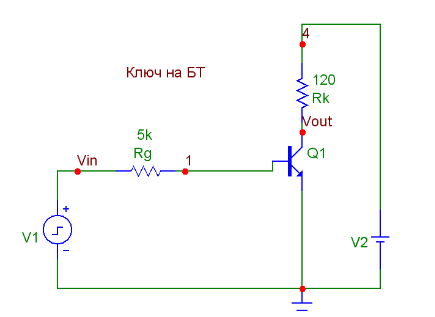
\includegraphics[width=0.7\linewidth]{image/BT_sh}
	\caption{Схема ключ на биполярном транзисторе с общим эмиттером без нагрузки}
	\label{fig:btsh}
\end{figure}

Далее получен график переходных процессов (рис. \ref{fig:btgrafper}).

\begin{figure}[H]
	\centering
	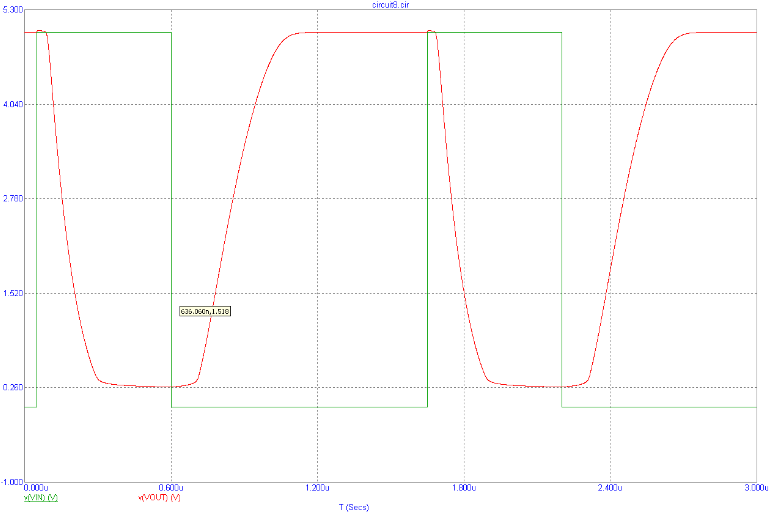
\includegraphics[width=0.7\linewidth]{image/BT_graf_per}
	\caption{График переходных процессов для БТ транзистора без нагрузки}
	\label{fig:btgrafper}
\end{figure}

С помощью инструмента «Вертикальная размерная линия» получаем $\Delta U$ (рис. \ref{fig:btgrafper1}).

$$\Delta U = 4.749 V$$

\begin{figure}[H]
	\centering
	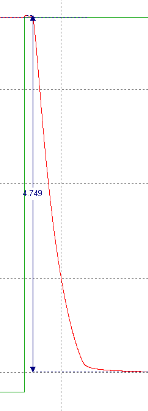
\includegraphics[width=0.2\linewidth]{image/BT_graf_per1}
	\caption{Применение инструмента «Вертикальная размерная линия» для измерения $\Delta U$}
	\label{fig:btgrafper1}
\end{figure}

На полученном графике переходных процессов определяем длительность фронтов $t^{01}_\phi$ и $t^{10}_\phi$.
Для этого необходимо рассчитать начало и конец нужного фронта.

\begin{itemize}
	\item Для переднего фронта: 
	\begin{itemize}
		\item Начало: $U^0 + \Delta * 10\%$
		\item Конец:  $U^1 - \Delta * 10\%$
	\end{itemize}
	
	\item Для заднего фронта: 
	\begin{itemize}
		\item Начало: $U^1 - \Delta * 10\%$
		\item Конец:  $U^0 + \Delta * 10\%$
	\end{itemize}
\end{itemize}

\begin{figure}[H]
	\centering
	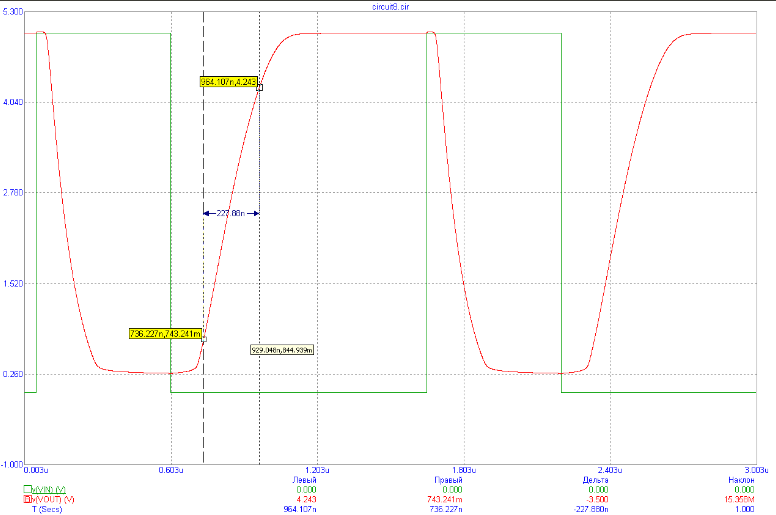
\includegraphics[width=0.7\linewidth]{image/BT_graf_t01}
	\caption{Измерение переднего фронта $t^{01}_\phi$}
	\label{fig:btgraft01}
\end{figure}

\begin{figure}[H]
	\centering
	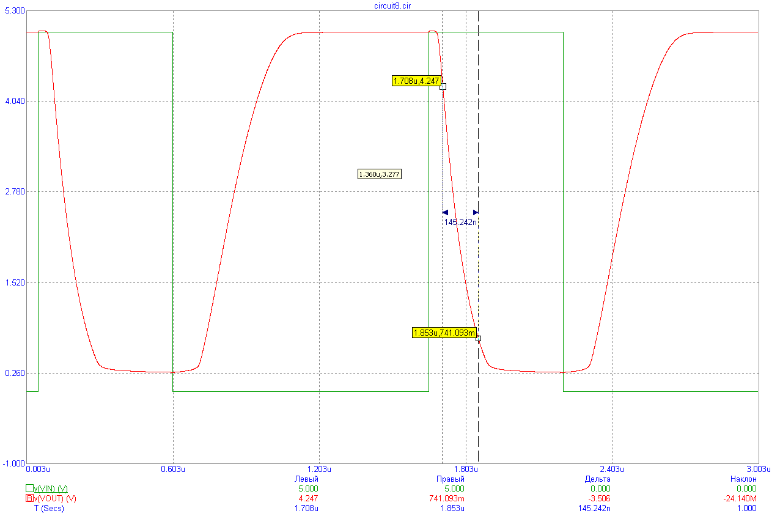
\includegraphics[width=0.7\linewidth]{image/BT_graf_t10}
	\caption{Измерение заднего фронта $t^{10}_\phi$}
	\label{fig:btgraft10}
\end{figure}

Из рисунков \ref{fig:btgraft01} и \ref{fig:btgraft10} получаем:

$$t^{01}_\phi = 227.88$$
$$t^{01}_\phi = 145.242$$

Далее измерим задержки переключения для $R_g = 5KOm$ и $R_g = 1KOm$, соответствующие графики представлены на рис. \ref{fig:btgrafzad5} и рис. \ref{fig:btgrafzad1}.

\begin{figure}[H]
	\centering
	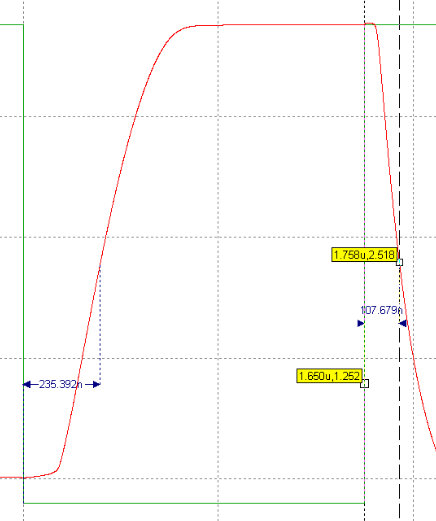
\includegraphics[width=0.4\linewidth]{image/BT_graf_zad_5}
	\caption{Значения $t^{01}_{zad}$ и $t^{10}_{zad}$ при $R_g = 5KOm$}
	\label{fig:btgrafzad5}
\end{figure}


\begin{figure}[H]
	\centering
	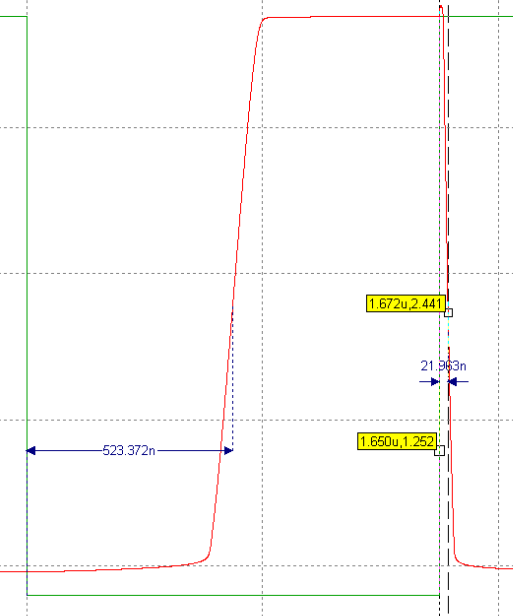
\includegraphics[width=0.4\linewidth]{image/BT_graf_zad_1}
	\caption{Значения $t^{01}_{zad}$ и $t^{10}_{zad}$ при $R_g = 1KOm$}
	\label{fig:btgrafzad1}
\end{figure}

Из графиков (рис. \ref{fig:btgrafzad5}, рис. \ref{fig:btgrafzad1}) получаем:

При $R_g = 5KOm$: $t^{01}_{zad} = 235.392ns$ и $t^{10}_{zad} = 107.679ns$

При $R_g = 1KOm$: $t^{01}_{zad} = 523.372ns$ и $t^{10}_{zad} = 21.963ns$

\textbf{Вывод:} при уменьшении сопротивления цепи базы $t^{01}_{zad}$ возрастает с $235ns$ до $523ns$, при этом  $t^{10}_{zad}$ наоборот падает с $108ns$ до $22ns$ 


Рассмотрим график анализа по постоянному току DC (рис. \ref{fig:btdc}), отметим на нем 2 точки и по их координатам посчитаем коэффициент передачи.

\begin{figure}[H]
	\centering
	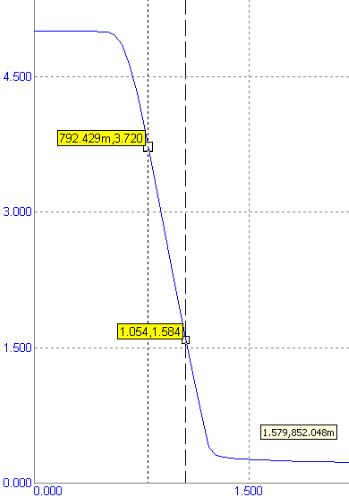
\includegraphics[width=0.4\linewidth]{image/BT_DC}
	\caption{График анализа по постоянному току DC}
	\label{fig:btdc}
\end{figure}

Коэффициент передачи равен тангенсу угла наклона прямой, найдем его из уравнения прямой $\dfrac{x-x_1}{x_2 - x_1} = \dfrac{y-y_1}{y_2 - y_1}$ получаем:

%$$\dfrac{x-729.429}{1054 - 729.429} = \dfrac{y-3.720}{1.584 - 3.720}$$

\begin{equation}
y = x * \dfrac{y_2 - y_1}{x_2 - x_1} - x_1 * \dfrac{y_2 - y_1}{x_2 - x_1} + y_1
\label{eq:line_bez_nagr}
\end{equation}

В формуле \ref{eq:line_bez_nagr} нас интересует коэффициент перед $x$, его абсолютное значение и будет коэффициентом $K$: 

\begin{equation}
K = \left|\dfrac{y_2 - y_1}{x_2 - x_1}\right|
\label{eq:K_bez_nagr}
\end{equation}

Подставим координаты точек из рис. \ref{fig:btdc} в формулу \ref{eq:K_bez_nagr}:

\begin{equation}
K = \left|\dfrac{1.584 - 3.720}{1.054 - 0.792} \right| = 8.15
\label{eq:K_bez_nagr_p}
\end{equation}


\subsection{Исследование ключа на биполярном транзисторе с нагрузкой}

Для исследования влияния на динамические параметры и формирующие свойства ключа параметров нагрузки добавим к схеме ключа на биполярном транзисторе нагрузку рис. \ref{fig:btshnagr}.

\begin{figure}[H]
	\centering
	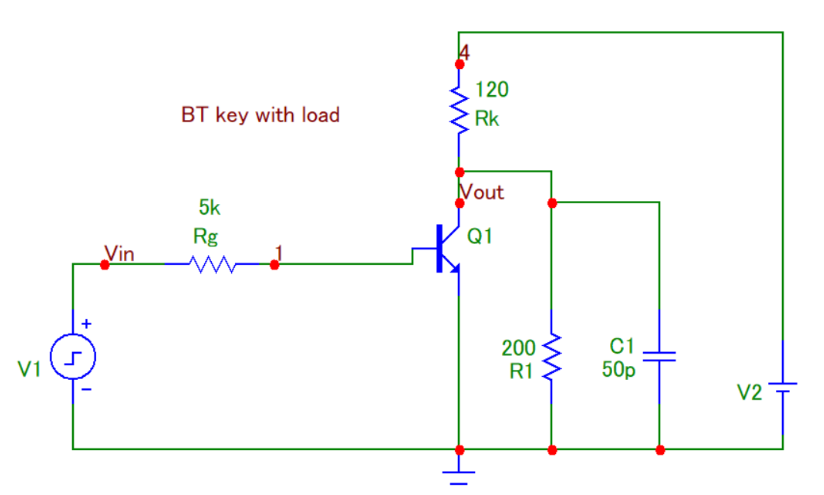
\includegraphics[width=0.7\linewidth]{image/BT_sh_nagr}
	\caption{Схема ключ на биполярном транзисторе с общим эмиттером с нагрузкой}
	\label{fig:btshnagr}
\end{figure}

\begin{figure}[H]
	\centering
	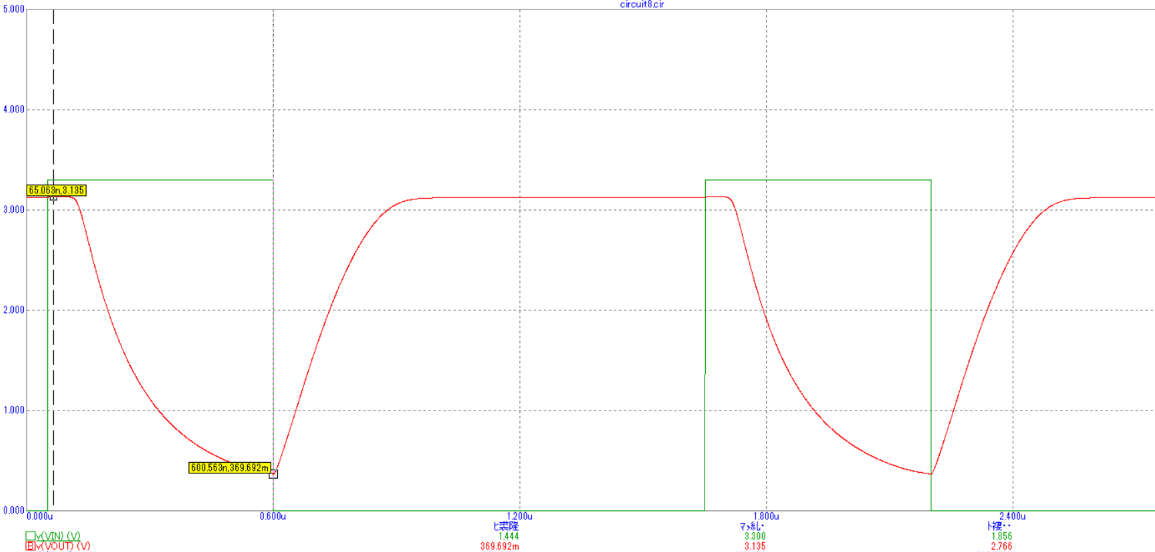
\includegraphics[width=0.7\linewidth]{image/BT_graf_nagr}
	\caption{График передаточной характеристики для ключа на биполярном транзисторе с нагрузкой}
	\label{fig:btgrafnagr}
\end{figure}

$U^0 = 0.369V$

$U^1 = 3.135V$

\begin{figure}[H]
	\centering
	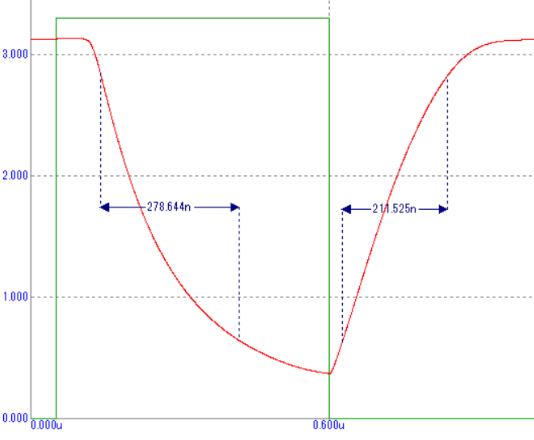
\includegraphics[width=0.4\linewidth]{image/BT_graf_nagr_fr}
	\caption{Измерение фронтов $t^{01}_{\phi}$ и $t^{10}_{\phi}$}
	\label{fig:btgrafnagrfr}
\end{figure}

\begin{figure}[H]
	\centering
	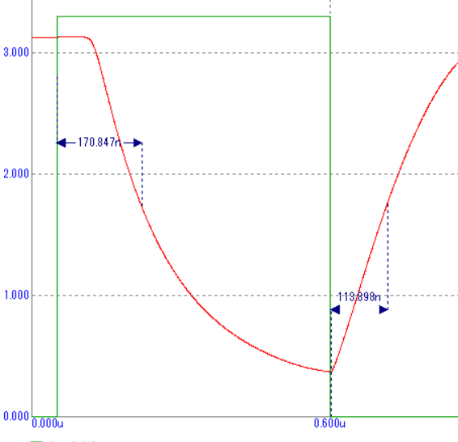
\includegraphics[width=0.4\linewidth]{image/BT_graf_nagr_zad}
	\caption{Измерение задержки переключения $t^{01}_{zad}$ и $t^{10}_{zad}$}
	\label{fig:btgrafnagrzad}
\end{figure}


На рисунках \ref{fig:btgrafnagrfr} и \ref{fig:btgrafnagrzad} представлены измерения фронтов и времени переключения соответственно для ключа на биполярном транзисторе с нагрузкой. 

Получаем следующие значения:

$t^{01}_{\phi} = 211.525ns$

$t^{10}_{\phi} = 278.644ns$

$t^{01}_{zad} = 119.898ns$

$t^{10}_{zad} = 170.847ns$

\begin{table}[H]
	\caption{Сравнение динамических характеристик ключа на биполярном транзисторе с нагрузкой и без}
	\centering
	\begin{tabular}{|l|c|c|c|c|}
		\hline
		& $t^{01}_{\phi}, ns$ & $t^{10}_{\phi}, ns$ & $t^{01}_{zad}, ns$ & $t^{10}_{zad}, ns$ \\ \hline
		без нагрузки & 227 & 145 & 235 & 107 \\ \hline
		с нагрузкой & 211 & 278 & 119 & 170 \\ \hline
	\end{tabular}

\label{tab:sr_har}
\end{table}


\textbf{Вывод: } появление нагрузки уменьшает динамические характеристики при включении ($t^{01}_{\phi}$ и $t^{01}_{zad}$) и увеличивает при выключении ($t^{10}_{\phi}$ и $t^{10}_{zad}$) ключа. Также можно заметить, что на графике динамических характеристик отсутствует пологая область характерная напряжению на выходе, равному $U^0$.



\section{Исследование ключа на КМДП транзисторах}
\subsection{Исследование ключа на КМДП транзисторах без нагрузки}

Построенная схема на КМДП транзисторах предсталена на рис. \ref{fig:kmdpsh}.

\begin{figure}[H]
	\centering
	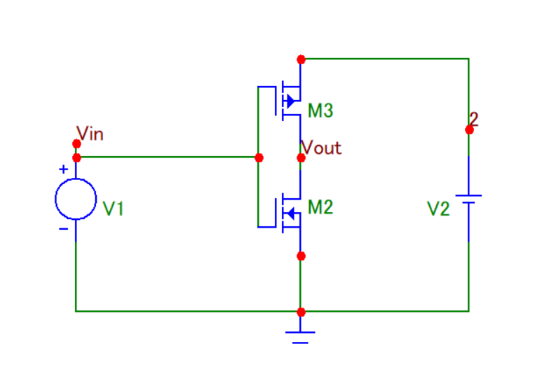
\includegraphics[width=0.7\linewidth]{image/KMDP_sh}
	\caption{Схема ключа на КМДП транзисторе без нагрузки}
	\label{fig:kmdpsh}
\end{figure}

%$t^{01}_{\phi}, ns$ & $t^{10}_{\phi}, ns$ & $t^{01}_{zad}, ns$ & $t^{10}_{zad}, ns$

Постоим график переходных процессов и на нем измерим $t^{01}_{\phi}$ и $t^{10}_{\phi}$ (рис.  \ref{fig:kmdpgraffr}).

\begin{figure}[H]
	\centering
	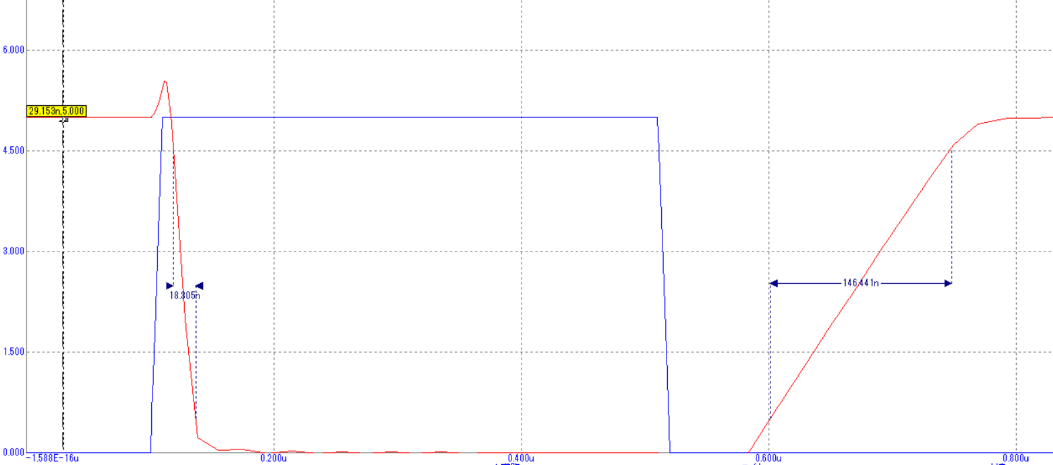
\includegraphics[width=0.7\linewidth]{image/KMDP_graf_fr}
	\caption{Измерение фронтов на КМДП транзисторе без нагрузки}
	\label{fig:kmdpgraffr}
\end{figure}

$U^0 = 5V$

$U^1 = 0V$

Далее измерим время задержки при переключении ключа $t^{01}_{zad}$ и $t^{10}_{zad}$ (рис. \ref{fig:kmdpgrafzad})

\begin{figure}[H]
	\centering
	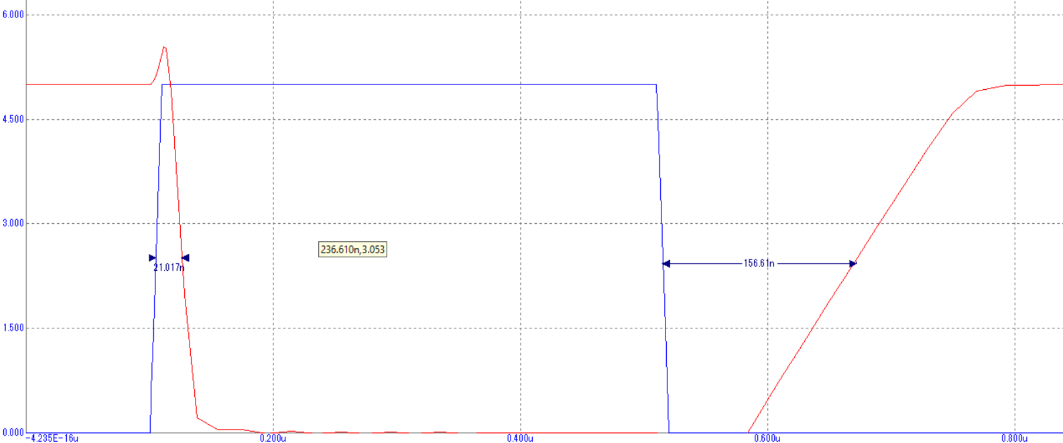
\includegraphics[width=0.7\linewidth]{image/KMDP_graf_zad}
	\caption{Измерение задержки на КМДП транзисторе без нагрузки}
	\label{fig:kmdpgrafzad}
\end{figure}

Получаем следующие динамические характеристики ключа на КМДП транзисторах:

$t^{01}_{\phi} = 146.441ns$

$t^{10}_{\phi} = 18.305ns$

$t^{01}_{zad} = 156.61ns$

$t^{10}_{zad} = 21.017ns$



\subsection{Исследование ключа на КМДП транзисторе с нагрузкой}

Добавим к схеме на КМДП транзисторах нагрузку, получим схему, которая представлена на рис. \ref{fig:kmdpshnagr}.

\begin{figure}[H]
	\centering
	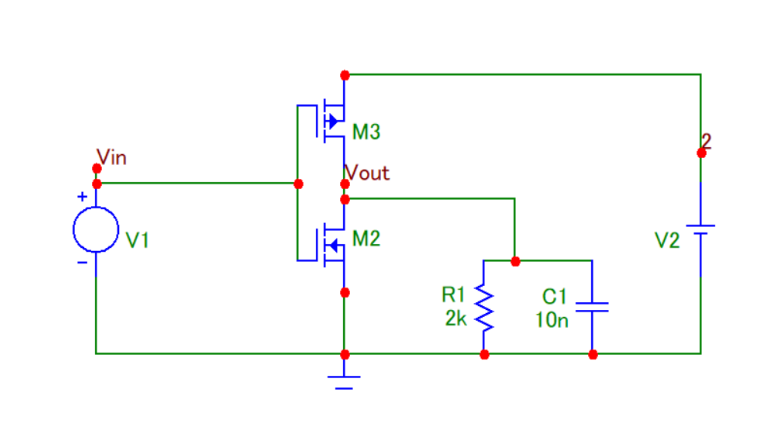
\includegraphics[width=0.7\linewidth]{image/KMDP_sh_nagr}
	\caption{Схема ключа на КМДП транзисторе без нагрузкой}
	\label{fig:kmdpshnagr}
\end{figure}

Постоим график переходных процессов и на нем измерим $t^{01}_{\phi}$ и $t^{10}_{\phi}$ (рис.  \ref{fig:kmdpgraffrnagr}).

\begin{figure}[H]
	\centering
	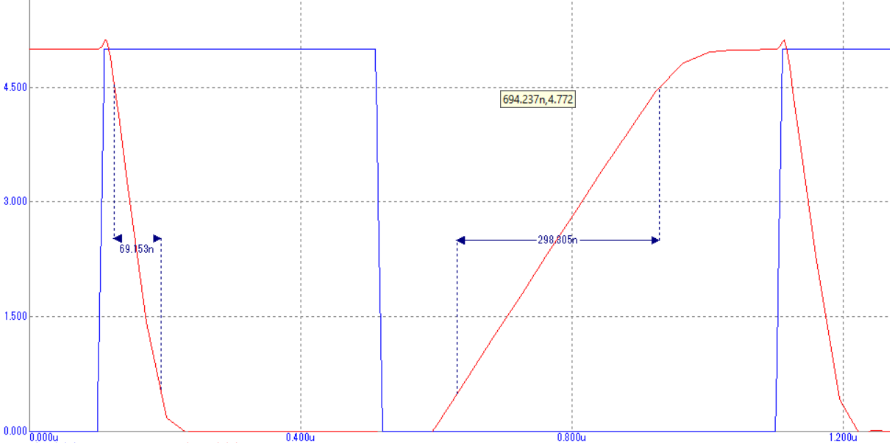
\includegraphics[width=0.7\linewidth]{image/KMDP_graf_fr_nagr}
	\caption{Измерение фронтов на КМДП транзисторе c нагрузкой}
	\label{fig:kmdpgraffrnagr}
\end{figure}

$U^0 = 5V$

$U^1 = 0V$

Далее измерим время задержки при переключении ключа $t^{01}_{zad}$ и $t^{10}_{zad}$ (рис. \ref{fig:kmdpgrafzadnagr})

\begin{figure}[H]
	\centering
	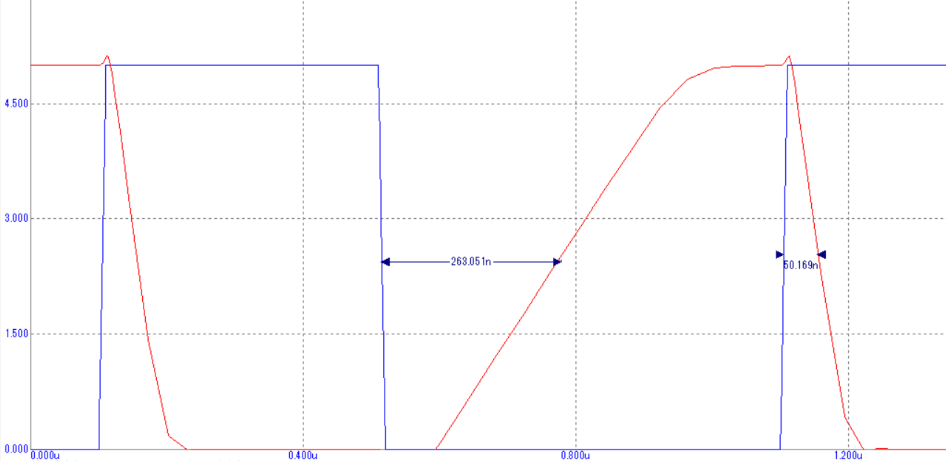
\includegraphics[width=0.7\linewidth]{image/KMDP_graf_zad_nagr}
	\caption{Измерение задержки на КМДП транзисторе с нагрузкой}
	\label{fig:kmdpgrafzadnagr}
\end{figure}

$t^{01}_{\phi} = 298.305ns$

$t^{10}_{\phi} = 69.153ns$

$t^{01}_{zad} = 263.051ns$

$t^{10}_{zad} = 50.169ns$

\textbf{Вывод: } Все динамические характеристики ключа выросли.

Построим график переходных процессов для ключа на КМДП транзисторах с нагрузкой (рис. \ref{fig:kmdpgrafper}).

\begin{figure}[H]
	\centering
	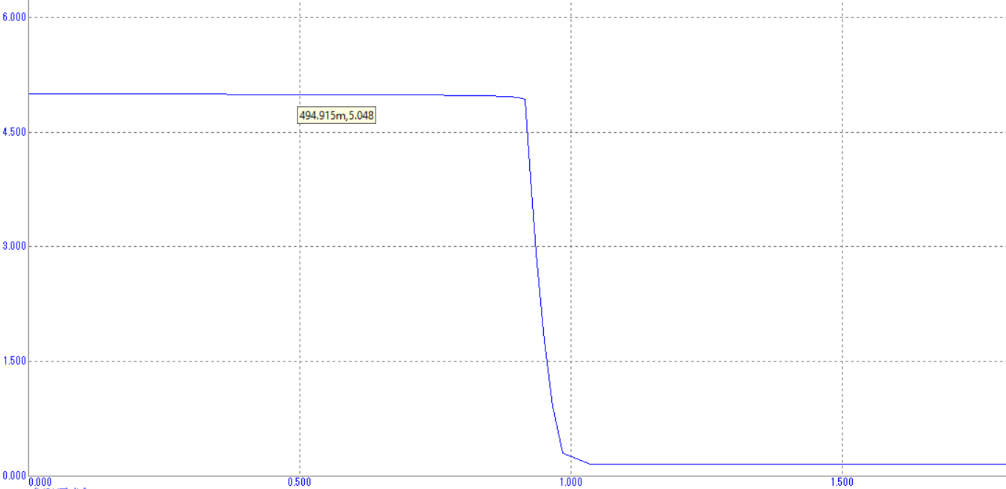
\includegraphics[width=0.7\linewidth]{image/KMDP_graf_per1}
	\caption{График переходных процессов }
	\label{fig:kmdpgrafper1}
\end{figure}

\begin{figure}[H]
	\centering
	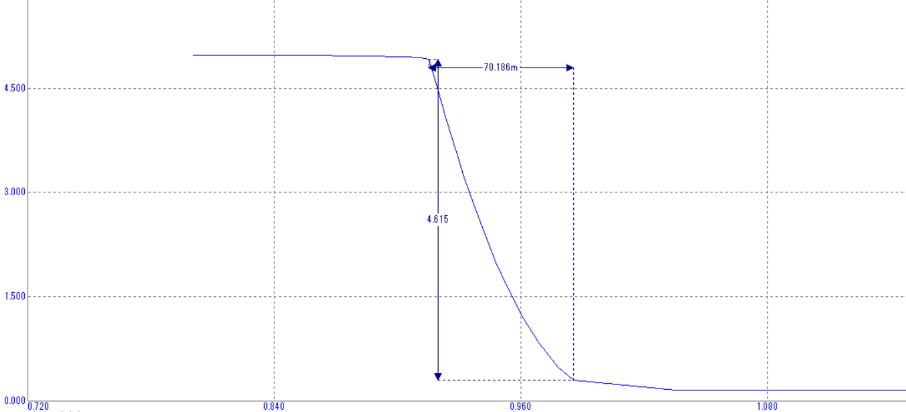
\includegraphics[width=0.7\linewidth]{image/KMDP_graf_per}
	\caption{Измерение коэффициента передачи}
	\label{fig:kmdpgrafper}
\end{figure}

$K = \dfrac{4.615}{0.070} = 65.93$

 \end{document} % конец документа






